\chapter{Results}
\label{sec:results}
%In previous chapters, there were introduced different methods available for selected use cases in research in biology and medicine. 
%\section{Virtual Infrastructure}
%\label{sec:resultsinfrastructure}
The pilot virtual infrastructure dedicated for research purposes, as proposed by the author of this thesis (3.), was established to consolidate and share resources among different projects. 
%The paper \cite{kulhanek2010c} \emph{Infrastructure for Data Storage and Computation in Biomedical Research} in Appendix~\ref{app:infrastructure} describes result of establishing the virtualization on physical infrastructure to share computational power among different platforms.
\section{Medical Image Sharing}
\label{sec:resultsimages}

The pilot infrastructure of several servers was installed in several institutions in Prague, Czech Republic. Globus Toolkit and Globus MEDICUS were installed on them,
the system connected with MEDIMED project integrates classical production system to share medical images with grid-based PACS system via the DICOM protocol. The grid-based system was tested with about 1300 DICOM records and enhanced with simple DICOMViewer available as web application. 
The grid-based solution allows to store large set of data records and manage replicas. The standard protocol to transfer data files gridFTP allows to effectively transfer parts of the files to the desired location from existing replicas within grid infrastructure to a desired location where an image processing can be performed. The grid-based solution brings robustness against the problems like single point of failure or bottleneck, where current systems of sharing medical images may suffer with such problems.

\section{Remote Voice Analysis}
\label{sec:resultsvoice}

RDP protocol was customized and support to transfer sound recording was implemented. A client plugin available for the Linux "rdesktop" application as well as for the Windows default "tsclient" application were customized to initiate sound recording and the raw data obtained from sound device is transferred to the custom RDP channel. The server plugin writes the data from the custom channel directly to the file in WAV format and concurently provides samples to the analytical application for real-time processing.
\begin{figure}[hbt]
    \centering
     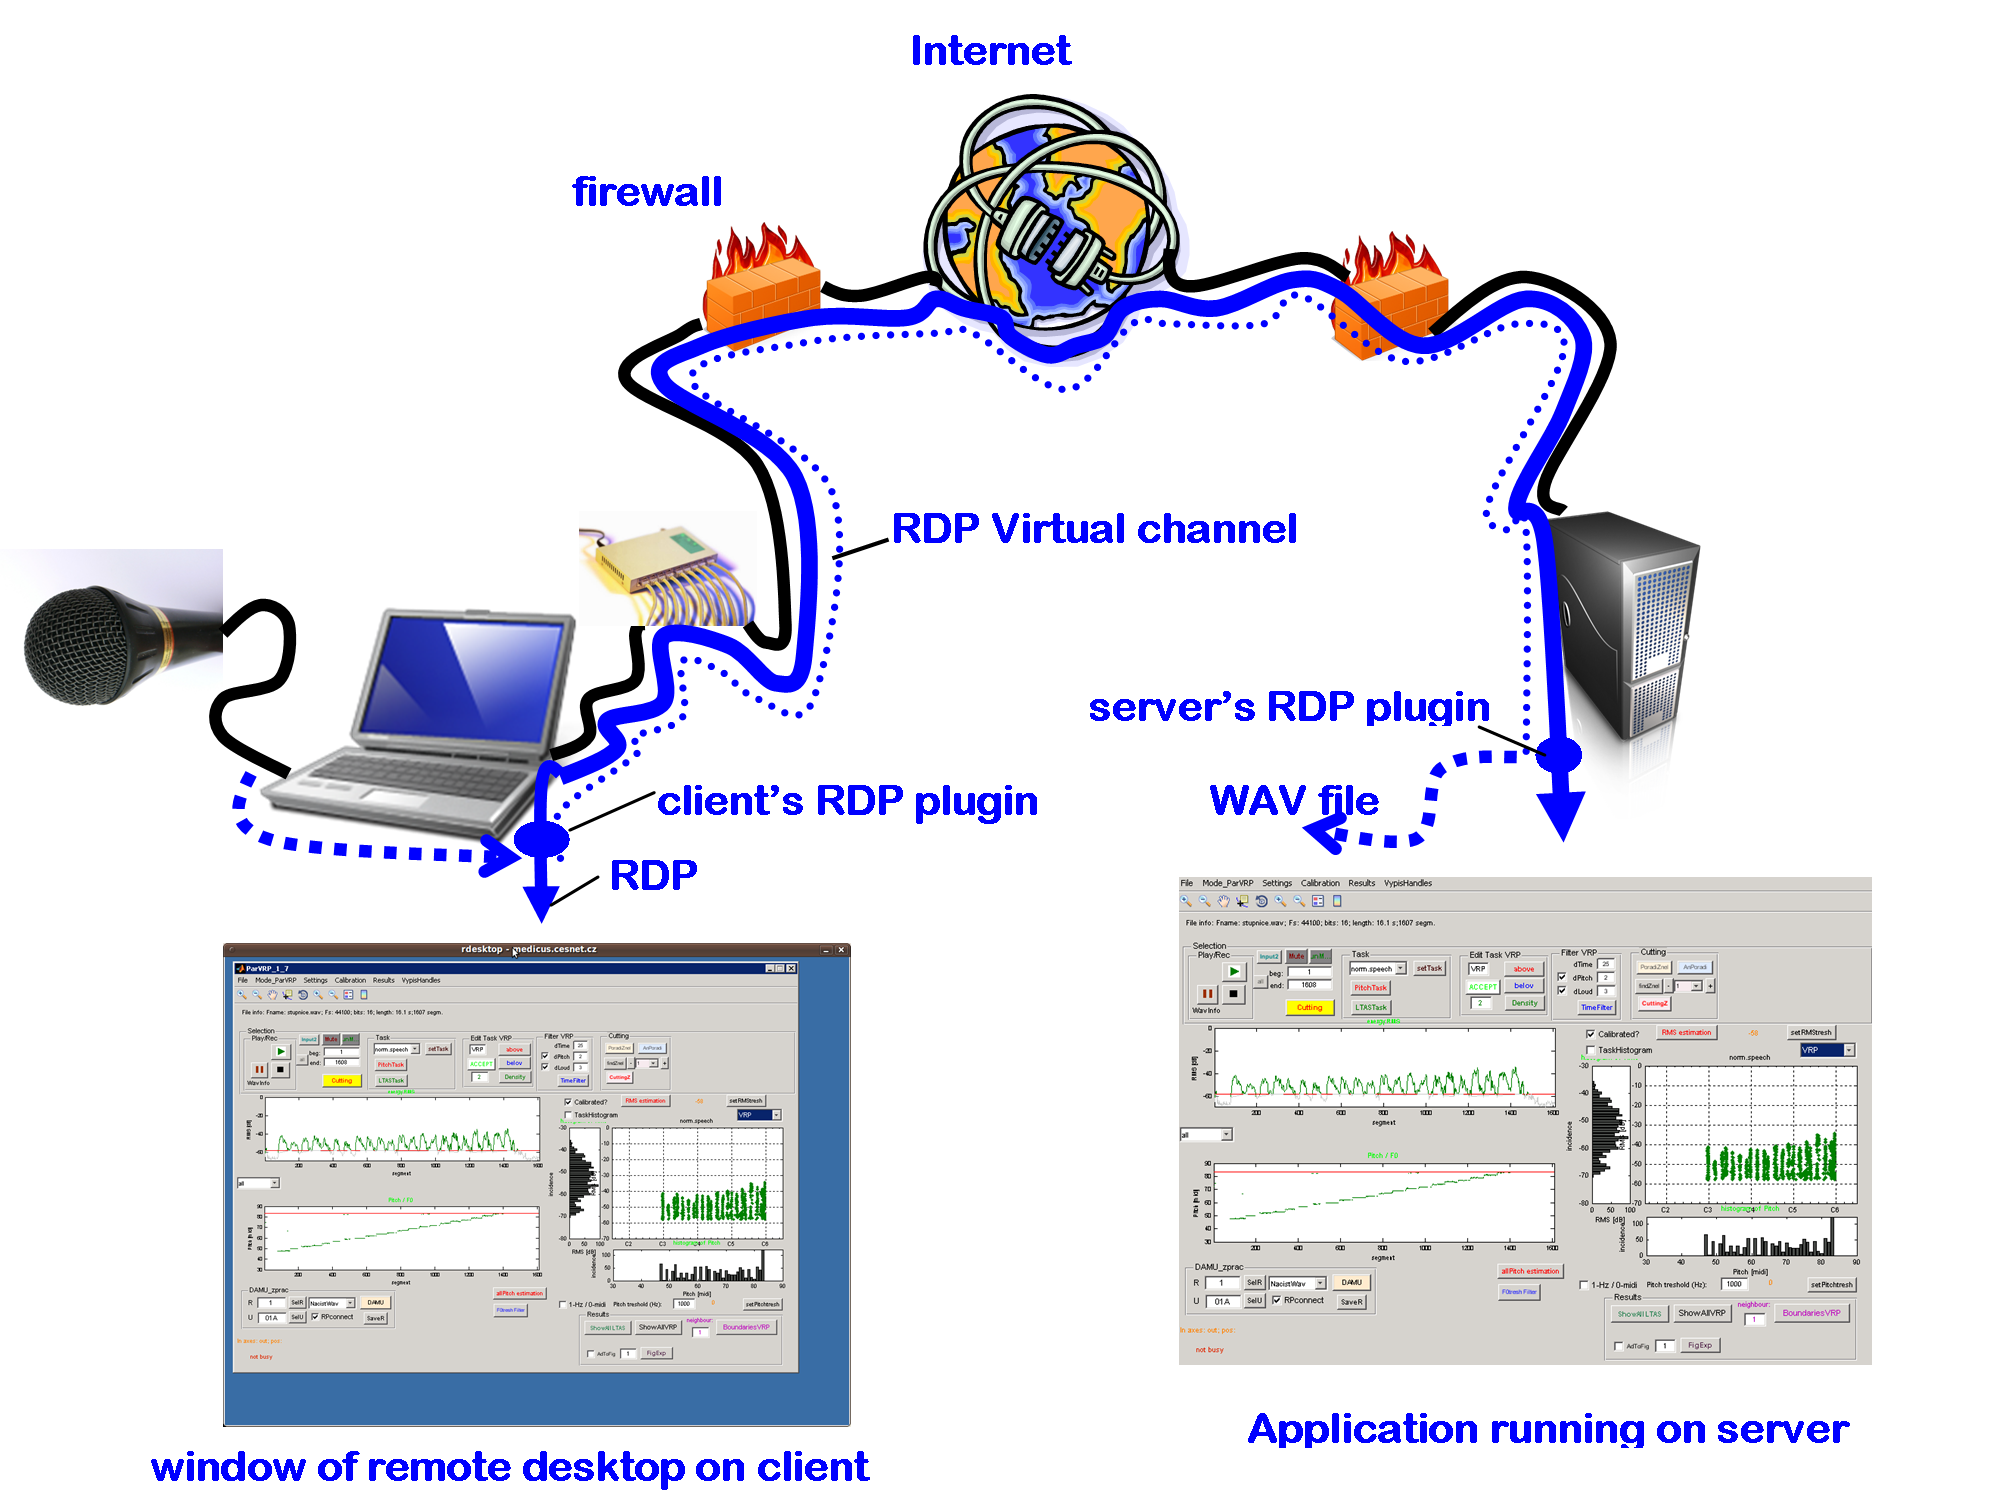
\includegraphics[width=0.75\textwidth]{schemasystemu.png}  
    \caption{Architecture of a system for remote voice analysis and RDP plugins for sound recording redirection.}
    \label{fig:architectureestimation}
\end{figure}

The default sound recording features of RDP protocol version 5.2 and 7.0 degrades sound quality transferred to the server application, furthermore, some samples of the sound were lost and sound become garbled or scratchy. The sound quality using the custom RDP channel is without loss of information and acceptable for further analysis. Additionally, the remote application with custom RDP plugin was packaged as a virtual machine template and can be provisioned on cloud computing infrastructure in case of the need.

The application allows to record the voice of patient, the voice signal is transfered to remote application where it is processed and analysed, the results are visualized in real-time. The application is now used by several voice therapists and voice pedagogues in different areas of the Czech Republic and Slovakia to analyze the voice non-invasive and to see e.g. the progress of the voice training methods.

\section{Computational Physiology}
\label{sec:resultsestimation}

The proposed architecture of the system for parameter estimation (Figure  \ref{fig:architectureestimation}) was influenced by the need of some interactivity and for the overall accessibility for users, which is fulfilled by the web UI. 

\begin{figure}[hbt]
    \centering
     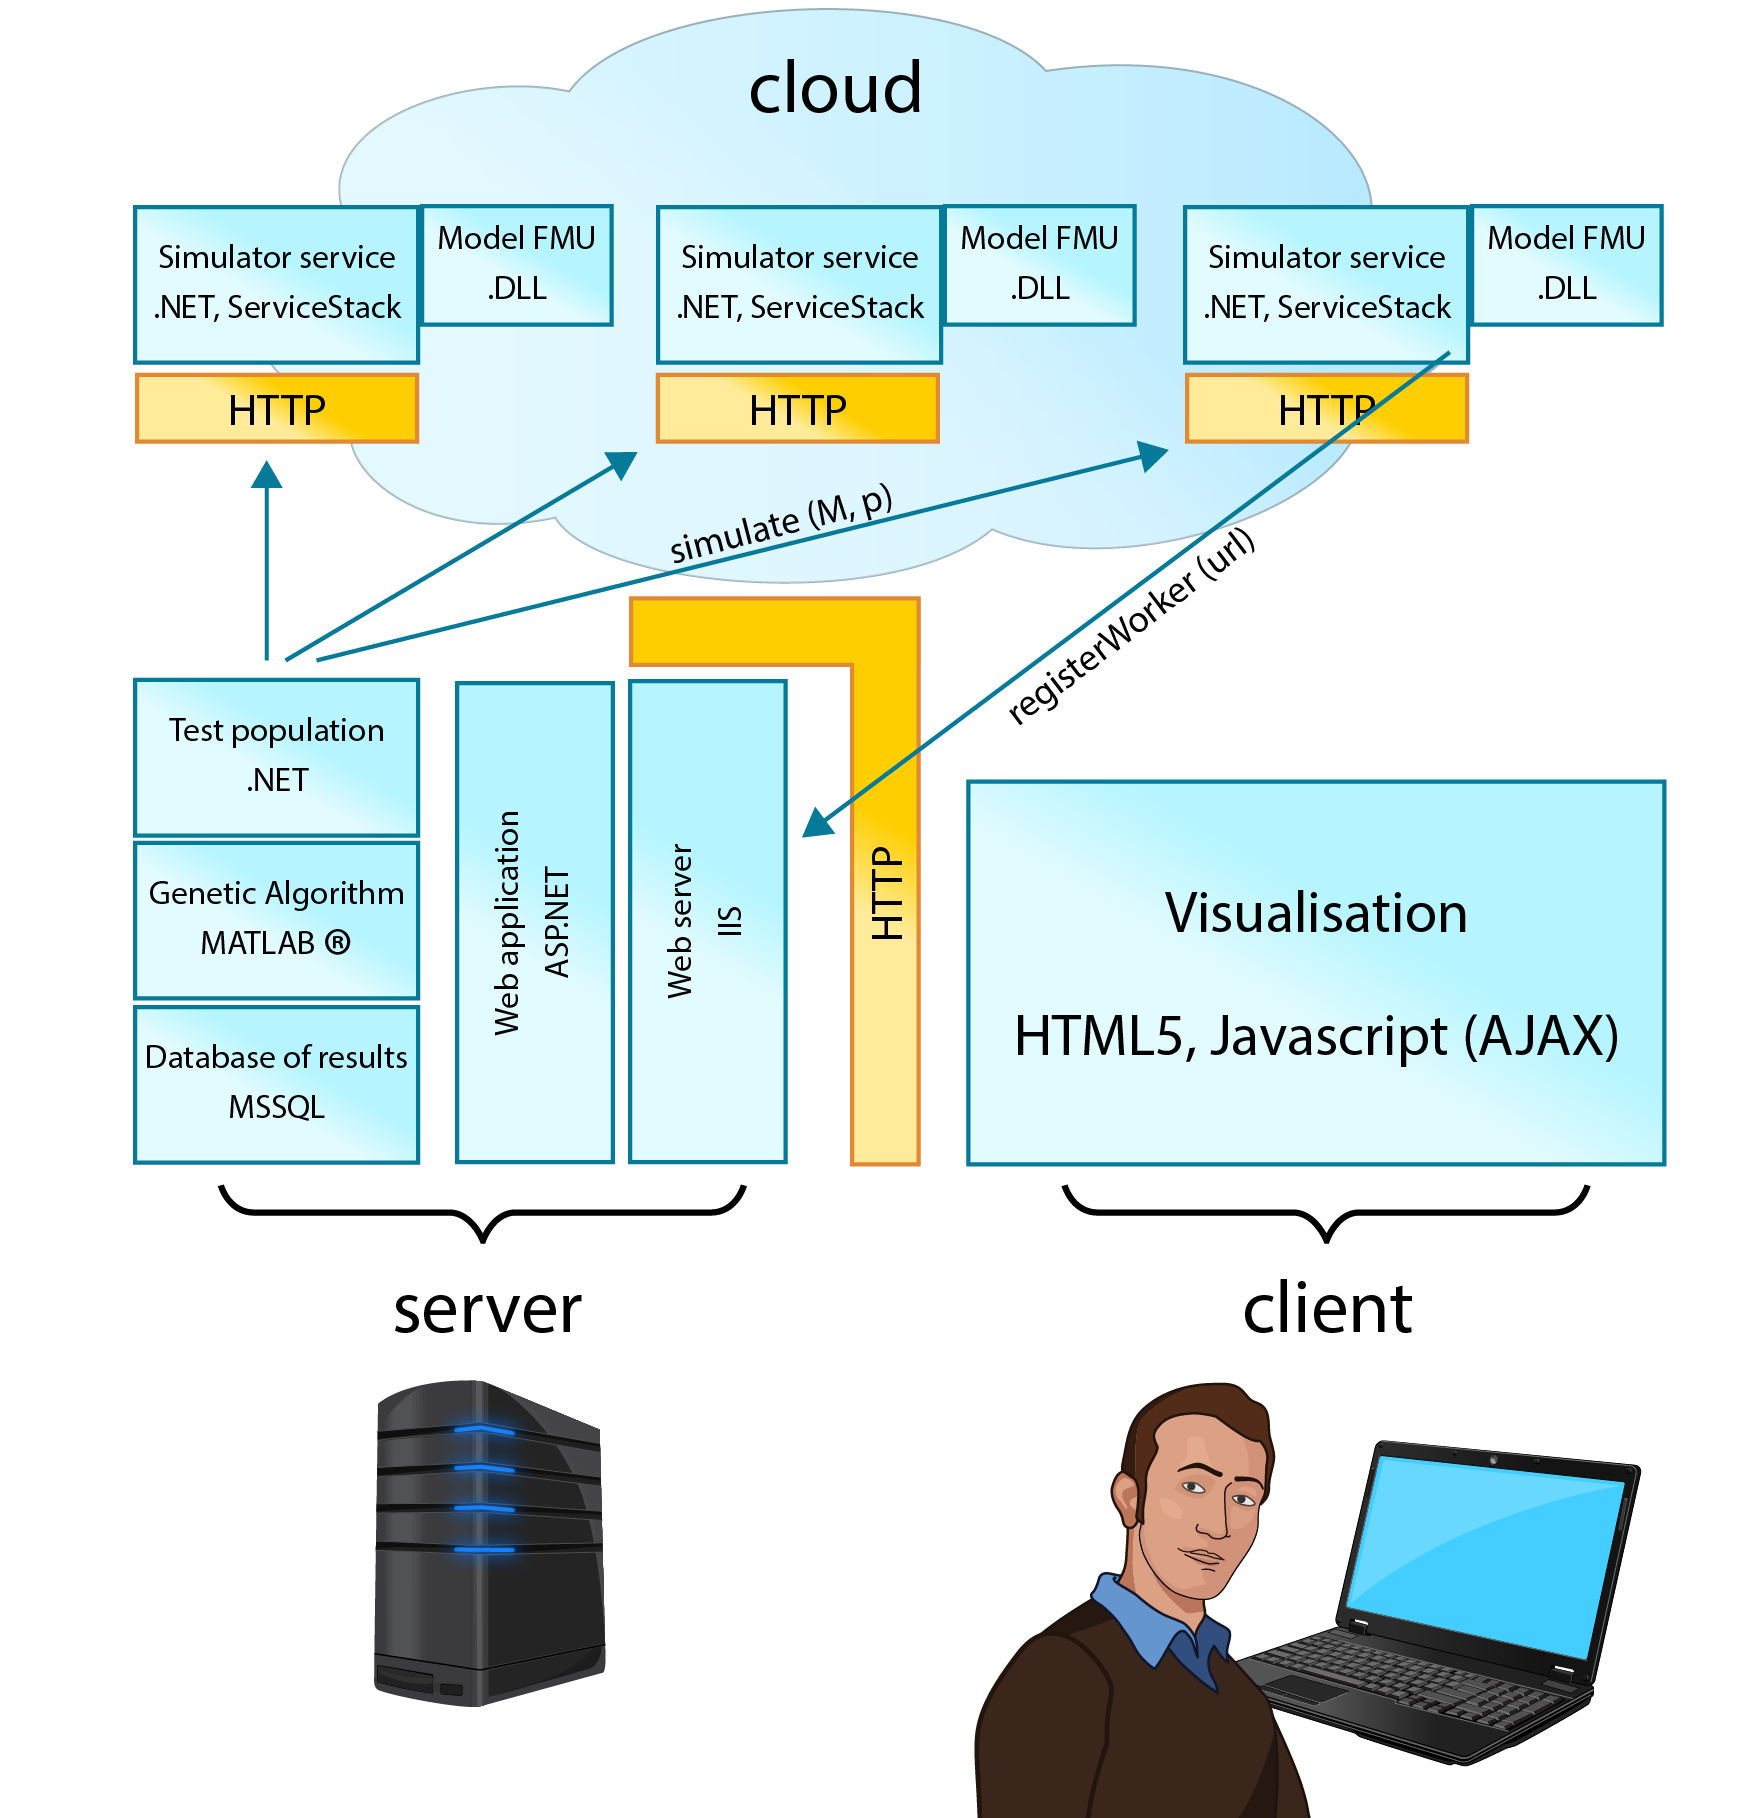
\includegraphics[width=0.75\textwidth]{../img/chapter3-architekturaestimation-01.png}  
    \caption{Architecture of a system that employs genetic algorithm and distributes the task \emph{simulate} into a cloud computing environment.}
    \label{fig:architectureestimation}
\end{figure}

The Modelica models is exported to standardized FMU and wrapped with custom code allowing, this can be called by custom application to perform simulation within needed constraints. In the time of writing this thesis, the most stable Modelica tool was Dymola version 2015\footnote{\url{http://www.dynasim.se} - Dymola tool, accessed March 2015}, and most stable export was to FMU for a MS Windows platform. 



\section{Parameter Sweep}
\label{sec:resultsboinc}